\documentclass{standalone}
\usepackage{tikz}
\begin{document}
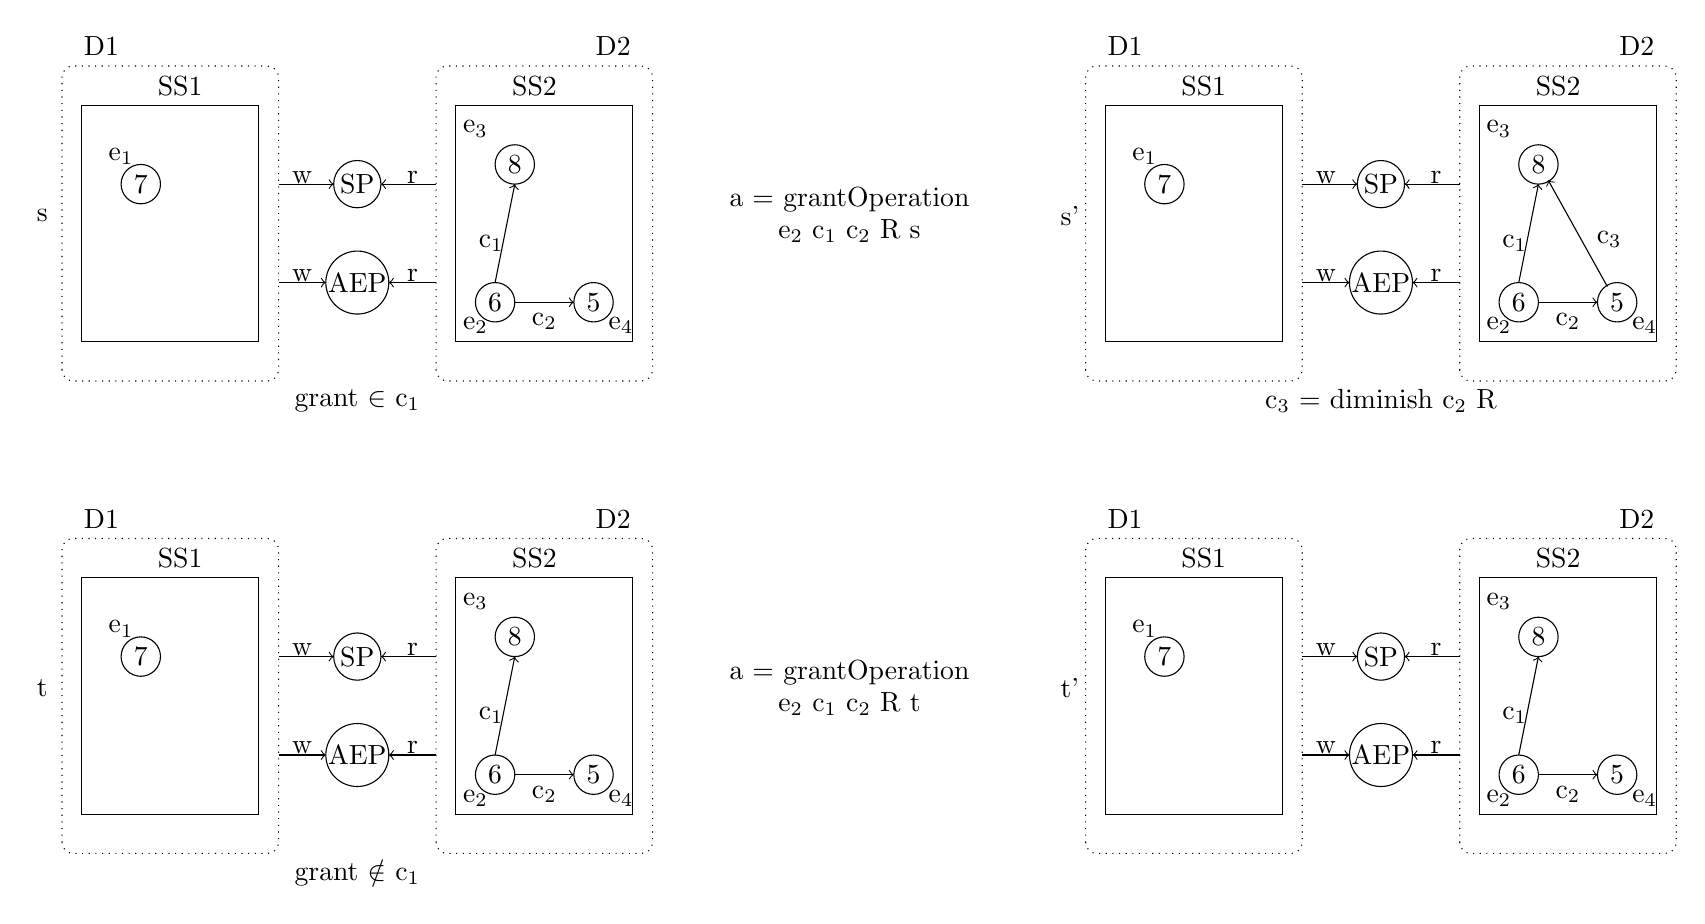
\begin{tikzpicture}
\node at (-0.25,1.6) {t};
\node at (1.5,3.25) {SS1};
\node at (0.5,3.75) {D1};
\node at (7,3.75) {D2};
\draw [black, dotted, rounded corners] (0,-0.5) rectangle (2.75,3.5);
\draw [black] (0.25,0) rectangle (2.5,3);
\draw [black, dotted, rounded corners] (4.75,-0.5) rectangle (7.5,3.5);
\draw [black] (5,0) rectangle (7.25,3);
\draw [black] (1,2) circle [radius=0.25] node {7};
\node at (0.75,2.35) {e$_1$};
\node at (6,3.25) {SS2};
\node at (5.25,2.7) {e$_3$};
\draw [black] (5.75,2.25) circle [radius=0.25] node {8};
\draw [black] (5.5,0.5) circle [radius=0.25] node {6};
\draw [black] (6.75,0.5) circle [radius=0.25] node {5};
\node at (5.25,0.2) {e$_2$};
\node at (7.1,0.2) {e$_4$};
\draw [->, black] (5.5,0.75) -- (5.75,2);
\draw [->, black] (5.75,0.5) -- (6.5,0.5);
\node at (5.45,1.25) {c$_1$};
\node at (6.125,0.25) {c$_2$};
\node at (3.75,-0.75) {grant $\notin$ c$_1$};
\node at (10,1.8) {a = grantOperation};
\node at (10,1.4) { e$_2$ c$_1$ c$_2$ R t};
\draw [black] (3.75,0.75) circle [radius=0.4] node {AEP};
\draw [black] (3.75,2) circle [radius=0.3] node {SP};
\draw [->, black] (2.75,0.75) -- (3.35,0.75);
\draw [<-, black] (4.15,0.75) -- (4.75,0.75);
\node at (3.05,0.84) {w};
\node at (4.45,0.84) {r};
\draw [->, black] (2.75,2) -- (3.45,2);
\draw [<-, black] (4.05,2) -- (4.75,2);
\node at (3.05,2.09) {w};
\node at (4.45,2.09) {r};

\node at (12.8,1.6) {t'};
\node at (13.5,3.75) {D1};
\node at (20,3.75) {D2};
\node at (14.5,3.25) {SS1};
\draw [black, dotted, rounded corners] (13,-0.5) rectangle (15.75,3.5);
\draw [black] (13.25,0) rectangle (15.5,3);
\draw [black, dotted, rounded corners] (17.75,-0.5) rectangle (20.5,3.5);
\draw [black] (18,0) rectangle (20.25,3);
\draw [black] (14,2) circle [radius=0.25] node {7};
\node at (13.75,2.35) {e$_1$};
\node at (19,3.25) {SS2};
\node at (18.25,2.7) {e$_3$};
\draw [black] (18.75,2.25) circle [radius=0.25] node {8};
\draw [black] (18.5,0.5) circle [radius=0.25] node {6};
\draw [black] (19.75,0.5) circle [radius=0.25] node {5};
\node at (18.25,0.2) {e$_2$};
\node at (20.1,0.2) {e$_4$};
\draw [->, black] (18.5,0.75) -- (18.75,2);
\draw [->, black] (18.75,0.5) -- (19.5,0.5);
\node at (18.45,1.25) {c$_1$};
\node at (19.125,0.25) {c$_2$};
\draw [black] (16.75,0.75) circle [radius=0.4] node {AEP};
\draw [black] (16.75,2) circle [radius=0.3] node {SP};
\draw [->, black] (15.75,0.75) -- (16.35,0.75);
\draw [<-, black] (17.15,0.75) -- (17.75,0.75);
\node at (16.05,0.84) {w};
\node at (17.45,0.84) {r};
\draw [->, black] (15.75,2) -- (16.45,2);
\draw [<-, black] (17.05,2) -- (17.75,2);
\node at (16.05,2.09) {w};
\node at (17.45,2.09) {r};

\node at (-0.25,7.6) {s};
\node at (1.5,9.25) {SS1};
\node at (0.5,9.75) {D1};
\node at (7,9.75) {D2};
\draw [black, dotted, rounded corners] (0,5.5) rectangle (2.75,9.5);
\draw [black] (0.25,6) rectangle (2.5,9);
\draw [black, dotted, rounded corners] (4.75,5.5) rectangle (7.5,9.5);
\draw [black] (5,6) rectangle (7.25,9);
\draw [black] (1,8) circle [radius=0.25] node {7};
\node at (0.75,8.35) {e$_1$};
\node at (6,9.25) {SS2};
\node at (5.25,8.7) {e$_3$};
\draw [black] (5.75,8.25) circle [radius=0.25] node {8};
\draw [black] (5.5,6.5) circle [radius=0.25] node {6};
\draw [black] (6.75,6.5) circle [radius=0.25] node {5};
\node at (5.25,6.2) {e$_2$};
\node at (7.1,6.2) {e$_4$};
\draw [->, black] (5.5,6.75) -- (5.75,8);
\draw [->, black] (5.75,6.5) -- (6.5,6.5);
\node at (5.45,7.25) {c$_1$};
\node at (6.125,6.25) {c$_2$};
\node at (3.75,5.25) {grant $\in$ c$_1$};
\node at (10,7.8) {a = grantOperation}; 
\node at (10,7.4) {e$_2$ c$_1$ c$_2$ R s};
\draw [black] (3.75,6.75) circle [radius=0.4] node {AEP};
\draw [black] (3.75,8) circle [radius=0.3] node {SP};
\draw [->, black] (2.75,6.75) -- (3.35,6.75);
\draw [<-, black] (4.15,6.75) -- (4.75,6.75);
\node at (3.05,6.84) {w};
\node at (4.45,6.84) {r};
\draw [->, black] (2.75,8) -- (3.45,8);
\draw [<-, black] (4.05,8) -- (4.75,8);
\node at (3.05,8.09) {w};
\node at (4.45,8.09) {r};

\node at (12.8,7.6) {s'};
\node at (13.5,9.75) {D1};
\node at (20,9.75) {D2};
\node at (14.5,9.25) {SS1};
\draw [black, dotted, rounded corners] (13,5.5) rectangle (15.75,9.5);
\draw [black] (13.25,6) rectangle (15.5,9);
\draw [black, dotted, rounded corners] (17.75,5.5) rectangle (20.5,9.5);
\draw [black] (18,6) rectangle (20.25,9);
\draw [black] (14,8) circle [radius=0.25] node {7};
\node at (13.75,8.35) {e$_1$};
\node at (19,9.25) {SS2};
\node at (18.25,8.7) {e$_3$};
\draw [black] (18.75,8.25) circle [radius=0.25] node {8};
\draw [black] (18.5,6.5) circle [radius=0.25] node {6};
\draw [black] (19.75,6.5) circle [radius=0.25] node {5};
\node at (18.25,6.2) {e$_2$};
\node at (20.1,6.2) {e$_4$};
\draw [->, black] (18.5,6.75) -- (18.75,8);
\draw [->, black] (18.75,6.5) -- (19.5,6.5);
\draw [->, black] (19.625,6.7) -- (18.874,8.05);
\node at (19.65,7.3) {c$_3$};
\node at (18.45,7.25) {c$_1$};
\node at (19.125,6.25) {c$_2$};
\node at (16.75,5.25) {c$_3$ = diminish c$_2$ R};
\draw [black] (16.75,6.75) circle [radius=0.4] node {AEP};
\draw [black] (16.75,8) circle [radius=0.3] node {SP};
\draw [->, black] (15.75,6.75) -- (16.35,6.75);
\draw [<-, black] (17.15,6.75) -- (17.75,6.75);
\node at (16.05,6.84) {w};
\node at (17.45,6.84) {r};
\draw [->, black] (15.75,8) -- (16.45,8);
\draw [<-, black] (17.05,8) -- (17.75,8);
\node at (16.05,8.09) {w};
\node at (17.45,8.09) {r};
\end{tikzpicture}
\end{document}
